\documentclass[UTF8]{ctexart}

%固定图片位置
\usepackage{float}

%插入超链接
\usepackage{url}

\usepackage{tikz,mathpazo}
\usetikzlibrary{shapes.geometric, arrows}
\usetikzlibrary{calc}

%\usepackage[affil-it]{authblk}

\usepackage{listings}
%插入代码的配置
\definecolor{CPPLight}  {HTML} {686868}
\definecolor{CPPSteel}  {HTML} {888888}
\definecolor{CPPDark}   {HTML} {262626}
\definecolor{CPPBlue}   {HTML} {4172A3}
\definecolor{CPPGreen}  {HTML} {487818}
\definecolor{CPPBrown}  {HTML} {A07040}
\definecolor{CPPRed}    {HTML} {AD4D3A}
\definecolor{CPPViolet} {HTML} {7040A0}
\definecolor{CPPGray}  {HTML} {B8B8B8}
\lstset{
	language=Matlab,                                     % 设置语言
    columns=fixed,    
    breaklines = true,   
    basicstyle=\small ,
    numbers=left,                                        % 在左侧显示行号
    %frame=none,                                          % 不显示背景边框
    backgroundcolor=\color[RGB]{245,245,244},            % 设定背景颜色
    keywordstyle=\color[RGB]{40,40,255}\bfseries,                 % 设定关键字颜色
    %commentstyle=\color{red!10!green!70}\textit,    % 设置代码注释的颜色
    numberstyle=\tiny\color{darkgray},           % 设定行号格式
    commentstyle=\it\color[RGB]{0,96,96},                % 设置代码注释的格式
    stringstyle=\rmfamily\slshape\color[RGB]{128,0,0},   % 设置字符串格式
    showstringspaces=false,                              % 不显示字符串中的空格                           
    %morekeywords={True,alignas,continute,friend,register,true,alignof,decltype,goto,
    %reinterpret_cast,try,asm,defult,if,return,typedef,auto,delete,inline,short,
    %typeid,bool,do,int,signed,typename,break,double,long,sizeof,union,case,
    %dynamic_cast,mutable,static,unsigned,catch,else,namespace,static_assert,using,
    %char,enum,new,static_cast,virtual,char16_t,char32_t,explict,noexcept,struct,
    %void,export,nullptr,switch,volatile,class,extern,operator,template,wchar_t,
    %const,false,private,this,while,constexpr,float,protected,thread_local,
    %const_cast,for,public,throw,std,rand},
    emph={access,and,break,class,continue,def,del,elif ,else,%
	except,exec,finally,for,from,global,if,import,in,i s,%
	lambda,not,or,pass,print,raise,return,try,while, imshow, subplot, figure,%
    log, fft2, fftshift, abs, size, rgb2gray, imread},
    emphstyle=\color{CPPViolet}\bfseries, 
    emph={[2]True, False, None, self},
	emphstyle=[2]\color{green},
	emph={[3]from, import, as},
	emphstyle=[3]\color{blue},
	upquote=true,
	morecomment=[s]{"""}{"""},
    morecomment=[s]{\%}{},
	%commentstyle=\color{orange}\slshape,
    commentstyle=\color{red!10!green!70}\textit,    % 设置代码注释的颜色
	emph={[4]1, 2, 3, 4, 5, 6, 7, 8, 9, 0},
	emphstyle=[4]\color{red},
	emph={[5]numpy, np, plt},
	emphstyle=[5]\color{red},
	literate=*{:}{{\textcolor{blue}:}}{1}%
	{=}{{\textcolor{blue}=}}{1}%
	{-}{{\textcolor{blue}-}}{1}%
	{+}{{\textcolor{blue}+}}{1}%
	{*}{{\textcolor{blue}*}}{1}%
	{!}{{\textcolor{blue}!}}{1}%
	{(}{{\textcolor{blue}(}}{1}%
	{)}{{\textcolor{blue})}}{1}%
	{[}{{\textcolor{blue}[}}{1}%
	{]}{{\textcolor{blue}]}}{1}%
	{<}{{\textcolor{blue}<}}{1}%
	{>}{{\textcolor{blue}>}}{1},%
    %{\%}{{\textcolor{green}\%}}{1},%
	framexleftmargin=0.1mm, framextopmargin=0.1mm, frame=shadowbox, rulesepcolor=\color{black},
}



\usepackage{geometry}
\geometry{left=2cm, right=2cm, top=1.2cm, bottom=1.2cm}

%得到引用的标题内容
\usepackage{nameref} 

%添加首行缩进,两个字符
\usepackage{indentfirst}
\setlength{\parindent}{2em}

%多行公式一个编号
\usepackage{amsmath}

%文献引用,标准类型为plain
%\usepackage[hyperref=true,backend=biber,sorting=none,backref=true]{biblatex}
%\addbibresource{ref.bib}
\bibliographystyle{plain}
\usepackage{cite}

\pagestyle{plain}

%跨页表格
\usepackage{multirow}
\usepackage{longtable,booktabs}
\usepackage{supertabular}
\usepackage{makecell}

%调整itemize等的间距
\usepackage{enumitem}


\usepackage{graphicx}
\usepackage{subfigure}

%超链接
\usepackage[linkcolor=yellow,citecolor=red,backref=page,hyperfootnotes=true]{hyperref}
\hypersetup{
bookmarks=true,
colorlinks=true,
linkcolor=black
}
\usepackage{tabularx} %This package must be placed after package {hyperref}, otherwise footnote marks are NOT treated as hyperlinks.


%引入了一些改进的数学环境,如align
\usepackage{amsmath}

\title{数字图像处理报告五:频域知识与$CNN$的结合}
\author{姓名:鲁国锐 \protect\newline
\and 学号:17020021031 \\
\and 专业:电子信息科学与技术}
\date{2020年4月22日}

\begin{document}
	\maketitle
	\renewcommand{\contentsname}{目录}
	\renewcommand{\listfigurename}{插图目录}
	\renewcommand{\listtablename}{表格目录}
	\renewcommand{\refname}{参考文献}
	\renewcommand{\abstractname}{摘要}
	\renewcommand{\indexname}{索引}
	\renewcommand{\tablename}{表}
	\renewcommand{\figurename}{图}
	
	
	
	\tableofcontents
	\newpage
	
	\hypersetup{
	bookmarks=true,
	colorlinks=true,
	linkcolor=red,
	urlcolor=blue
	}
	\section{题目描述}
	\indent 对比传统图像复原方法和深度学习图像复原方法的特点和各自优势,尽可能给出详细分析。

			
%			\begin{figure}[H]
%				\centering 
%				
\includegraphics[scale=0.4]{org_img.png} 
%				\caption{原图及其傅里叶变换} 
%				\label{problem_img}
%			\end{figure}
		


	
	\section{传统图像复原方法}\label{traditional_methods}
        \indent 所谓传统的图像复原方法,在这里指的就是在深度学习出现以前的方法。
        
        \subsection{特点}
            \indent 关于传统方法的特点,具体而言可以归结为以下几点:
    			
                \begin{enumerate}[leftmargin=50pt]
    				\item 需要有退化现象的某种先验知识\cite{digit_image_Gonzalez};
    				\item 人为观察、实验和建模\cite{digit_image_Gonzalez};
    				\item 需要技术人员有比较丰富的图像处理经验;
    				\item 需要具体问题具体分析。
    			\end{enumerate}                
            
            \indent 可以看出,传统复原方法的最大特点就是“人的参与”。不论是对于问题的分析还是实际的操作,都高度依靠技术人员的背景知识以及经验,往往需要人来分析问题,挑选滤波器,难以做到自动化处理。
            
            \indent 另外,每遇到一个新的问题,都需要技术人员针对其再分析一遍,人为设计一套新的流程来处理它,比较耗时。
            
        \subsection{优势}\label{advantages_of_traditional_methods}
            \indent 传统图像复原方法的优势,可以总结为以下两点:
    			\begin{enumerate}[leftmargin=50pt]
    				\item 计算量小,对处理器要求低,容易移植到移动设备上;
    				\item 可解释性好\footnotemark[1]。
    			\end{enumerate}
      
            \indent 第一点可以说是传统方法最大的优点,也是它为何能在这个以大数据和深度学习为主导的时代中继续发光发热的原因。深度学习主要基于复杂的神经网络,难以做到轻量级,所以无论是训练还是使用,都对处理器有较高的要求,移动设备往往无法承担如此巨大的计算量,更不用说实时处理。
            
            \indent 第二点\footnotemark[1]主要是针对于深度学习而言的,由于通过传统方法得到的算法每一步都是有人来掌控的,所以我们很清楚一个算法每一步都做了什么。而深度学习则不然,它更像是一个黑盒子,人们只管设计出一个网络结构和$loss$函数,再经大数据训练就能得到一个非常好的结果。这是深度学习的优势,也是它的劣势,在这一节中主要讨论它所带来的问题。
            
            \indent 当电脑运行算法得到了一个结果后,很多时候我们不光只关注它的正确性,还会在意这个结果是如何得到的。一个算法究竟是依据什么内容得出了该结果?在某些领域(如医疗、金融等)这一点至关重要,因为它直接决定了人们是否相信这个算法。可惜的是,深度学习在这一点上始终难以做到“有理有据”。人们通过使用它能轻松得到相当不错的效果,但却无法在它出错时给出针对性的解释和解决方法,更无法提前预估出神经网络可能会犯哪些错,从而防患于未然。而当它犯的错极有可能导致相当严重的后果时,人们很难说服自己去相信深度学习——尽管它在很多场景下的成功率早已超过了人类。
            
            \indent 一言以蔽之,“要么不犯错,要么犯大错”,这便是深度学习相对于传统方法而言的另一大劣势。只不过在本文所讨论的图像复原这一应用中,这一劣势似乎并不致命而已。
            
            \footnotetext[1]{这一点的写作主要参考了上海交通大学张拳石教授的知乎专栏:\url{https://zhuanlan.zhihu.com/p/30074544}}
    
    
    \section{基于深度学习的图像复原方法}\label{DeepLearning_methods}
    
        \subsection{特点}
            \indent 深度学习图像复原方法的特点可以归结为以下几点:
            
    			\begin{enumerate}[leftmargin=50pt]
    				\item 由数据驱动,依靠大数据训练来使模型自动学习到知识(分布);
    				\item 对操作者的先验知识、经验等要求较低;
    				\item 可以直接解决比较广泛的问题。
    			\end{enumerate}
            
            \indent 不难看出,深度学习相对于传统方法来说,最大的特点是减少了“人的参与”。正如\ref{advantages_of_traditional_methods}节中所说的,技术人员只需要找到合适的数据集,设计出一个合理的网络结构和$loss$函数,就可以训练出一个表现优异的模型。并且在数据量较大的情况下,可以一次性解决一类或多类问题。比起传统方法需要技术人员事事亲力亲为,深度学习在很多事情上达到了自动化处理的效果。
    			
%    			\begin{figure}[htbp]
%    				\centering 
%         			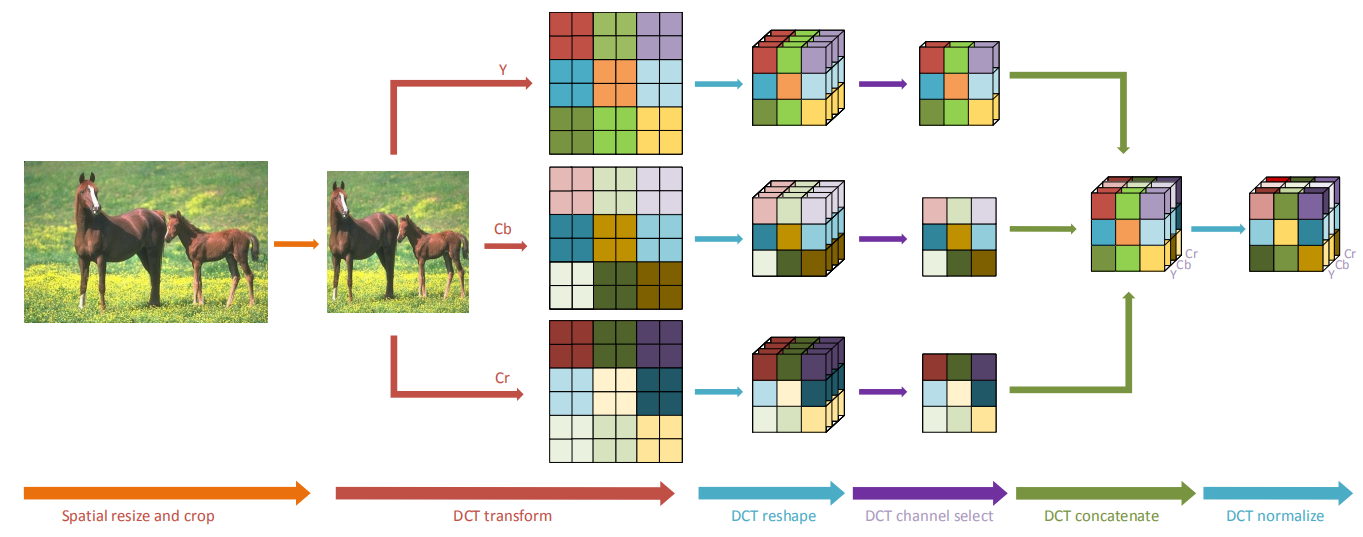
\includegraphics[scale=0.5]{pre-processing.png} 
%    				\caption{预处理流程示意图} 
%    				\label{pre-processing}
%    			\end{figure}
        \subsection{优势}
            \indent 基于深度学习的图像复原方法,其优势也是相当明显的:
         
            
    			\begin{enumerate}[leftmargin=50pt]
    				\item 降低了操作门槛;
                    \item 缩短了开发周期;
                    \item 在数据充足的情况下往往能取得不错的效果。
    			\end{enumerate}
                
            \indent 深度学习将人们从繁琐的观察、建模过程中解放了出来,在提升了效果的同时,还大大缩短了开发周期。这在很大程度上得益于它的“黑盒子”这一特性,使人们不用对更底层的原理给予太多关注,只要按照一定的流程,无需太多的数学物理知识即可为很多问题提供一个漂亮的解决方案。
                
            
%        \nocite{digit_image_Gonzalez}
%        \nocite{signal_and_system}
%        \nocite{discrete-time_signal_processing}



		

            


%			\indent 采取\ref{数字相机成像原理}节的方式,我们也可以把线性扫描相机的原理概括为以下$3$个步骤:
%			\begin{enumerate}[leftmargin=50pt]
%				\item 由条带传感器成像,给出一幅图像一行(或一列)的像素值;
%				\item 沿垂直于传感器带的方向移动一小段距离;
%				\item 重复步骤$1$和步骤$2$,直至整幅图像全部成像完毕。
%			\end{enumerate}

%		\begin{enumerate}[leftmargin=50pt]
%			\item 所成图像在垂直方向上的大小不受限制;
%			\item 能够通过提高扫描频率达到非常高的分辨率;
%			\item 使用起来灵活方便等
%		\end{enumerate}
		
%	\section{实验验证}
%        \subsection{实验思想}
%            \indent 从前面的分析可以看出,频谱图上的谱线与空间域中像素变化的方向及剧烈程度有关。从这个角度出发,如果把空间域图像转一个角度,频谱图中的谱线相应地也应该旋转相同的角度。我们将在之后的两个小节中对这个猜想进行验证。
%        \subsection{实验代码}
%            	\begin{lstlisting}[language=Matlab,caption={实验代码},label={broadcast.cpp}]
%% reference: https://blog.csdn.net/jiugedexiaodi/article/details/79705308
%
%
%
%img = imread('C:\Users\Asus-\Desktop\数字图像\report\04\rotate45.png');
%img = rgb2gray(img);
%
%% 将图像的数据格式转换为double型的,此时图像的数值范围由原来的[0,255],
%% 变成了[0,1],其实不进行转换的话,也可以进行傅里叶变换,
%% 只是傅里叶变换后的图像会有所不同
%img=im2double(img);
%
%% size(img)
%
%F = fft2(img);
%F = fftshift(F);
%F = abs(F);
%
%% 傅里叶变换后模值差异非常大,低频直流远远大于高频
%% 不加这一句变换后的结果只能看到中间有一个亮点
%T = log(1+F);
%figure(1)
%subplot(1, 2, 1)
%imshow(img)
%subplot(1, 2, 2)
%% 后面的[],表示对图像做了一个类似于归一化的操作,
%% 防止傅里叶变换后模值差异太大
%imshow(T, [])
%            	\end{lstlisting}
                

        
%            \begin{figure}[htbp]
%            	\centering 
%                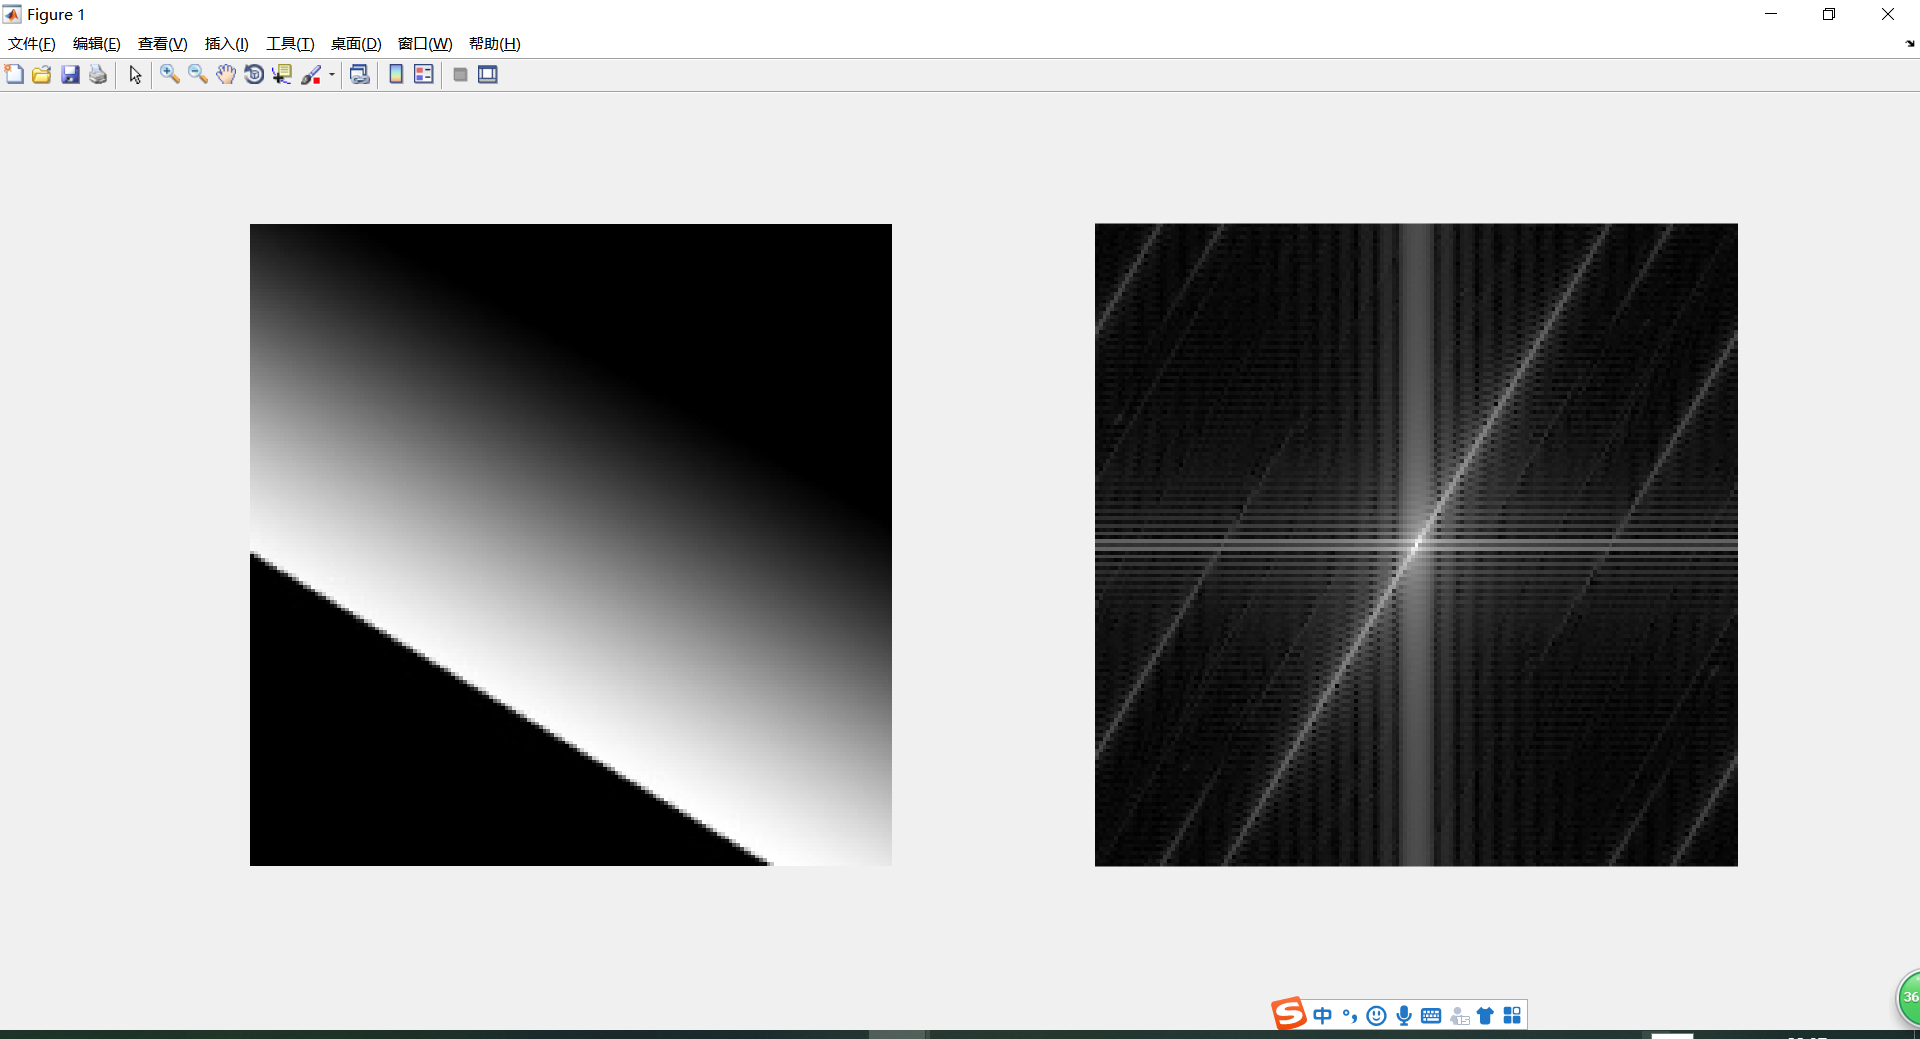
\includegraphics[scale=0.4]{result.png} 
%            	\caption{实验结果} 
%            	\label{result}
%            \end{figure}

            


	\section{总结}
		\indent 本文总结了部分传统图像复原方法和深度学习图像复原方法的特点及优势,并尽力给出了相应的分析。
        
        \indent 综合来看,深度学习是一个更为高级的工具,能够为我们解决大量过去难以企及的问题。但这并不意味着传统方法的过时甚至淘汰,在许多场景下,传统方法依然有着不可忽视的力量。就像高铁、飞机虽已普及,但自行车等传统交通工具依然能得到广泛的应用。根据需求决定方案,这才是解决问题的最终思路。
%			\begin{figure}[H]
%				\centering 
%				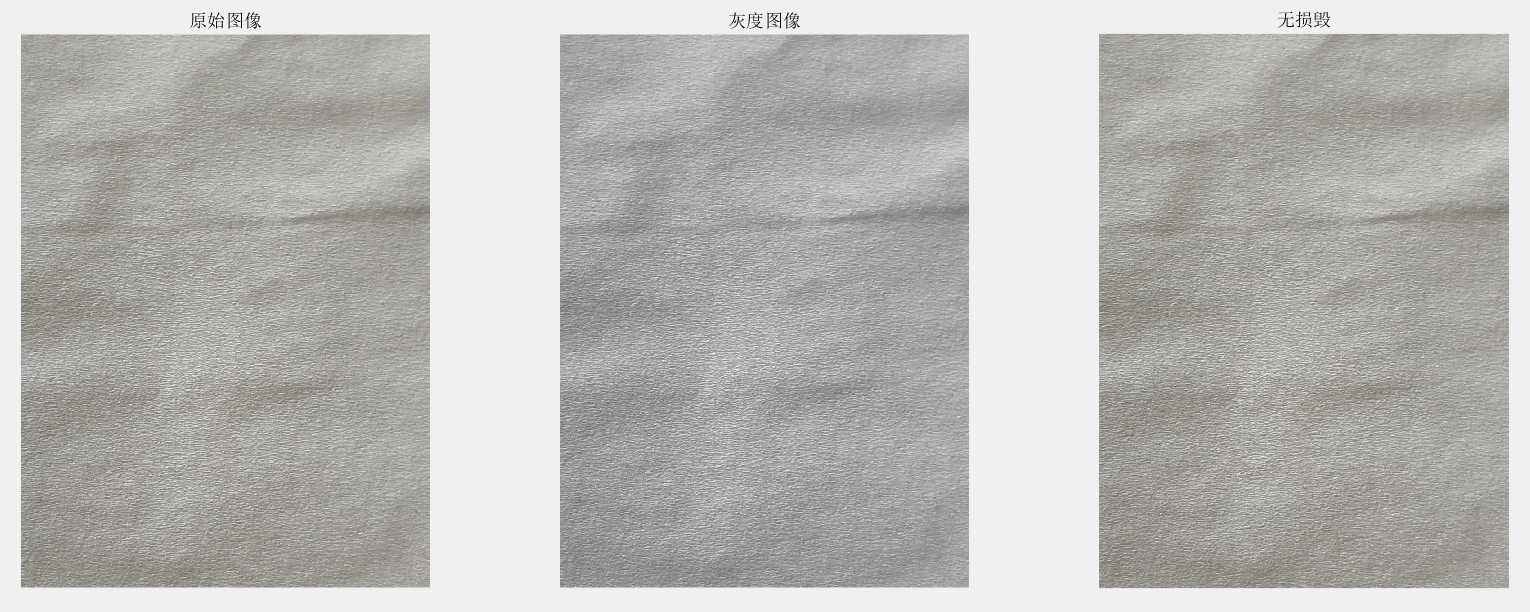
\includegraphics[scale=0.4]{res4.png} 
%				\caption{结果4} 
%				\label{res4}
%			\end{figure}
		

		
%			\begin{figure}[H]
%				\centering 
%				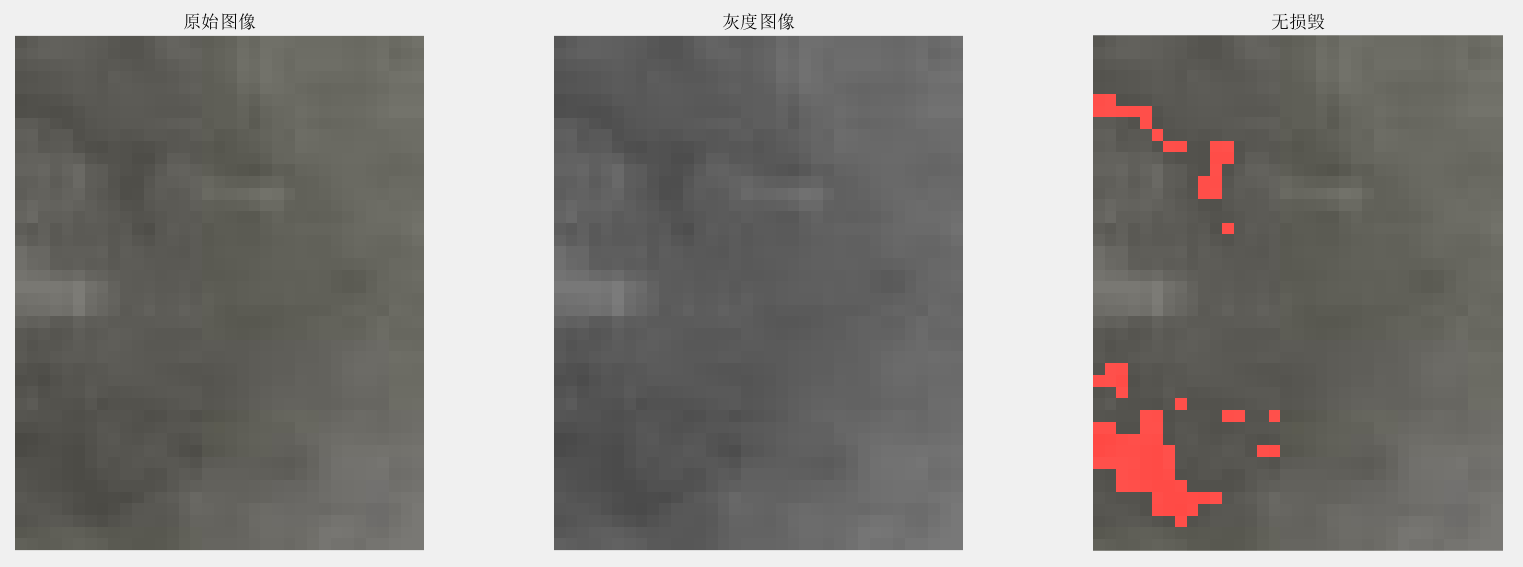
\includegraphics[scale=0.4]{res6.png} 
%				\caption{结果6(截取自结果5的阴影部分)} 
%				\label{res6}
%			\end{figure}
	
	
% 中文文献多个作者用中文逗号“,”连接
%\bibliography{ref.bib}
%\bibliographystyle{abbrv}
\bibliography{ref.bib}


\end{document}